%%%%%%%%%%%%%%%%%%%%%%%%%%%%%%%%%%%%%%%%%
% Beamer Presentation
% Standard LaTeX Template used for creating presentation of Firebird-V Robot and other tutorials. 
% Author: Saurav Shandilya (e-Yantra Team)
% Reference: www.LaTeXTemplates.com Version 1.0 (10/11/12)
%
%%%%%%%%%%%%%%%%%%%%%%%%%%%%%%%%%%%%%%%%%

%----------------------------------------------------------------------------------------
%	PACKAGES AND THEMES
%----------------------------------------------------------------------------------------
		
\documentclass[table,10pt,red]{beamer}	% First line -- Define document class as Beamer which is used for creating presentation using Latex
\setbeamercolor{alerted text}{fg=blue} 	% Sets color of highlighted text during presentation.  
 

% The Beamer class comes with a number of default slide themes
% which change the colors and layouts of slides. Below this is a list
% of all the themes, uncomment each in turn to see what they look like.

%\usetheme{default}
%\usetheme{AnnArbor}
%\usetheme{Antibes}
%\usetheme{Bergen}
%\usetheme{Berkeley}
\usetheme{Berlin}		%used theme in present documents.
%\usetheme{Boadilla}
%\usetheme{CambridgeUS}
%\usetheme{Copenhagen}
%\usetheme{Darmstadt}
%\usetheme{Dresden}
%\usetheme{Frankfurt}
%\usetheme{Goettingen}
%\usetheme{Hannover}
%\usetheme{Ilmenau}
%\usetheme{JuanLesPins}
%\usetheme{Luebeck}
%\usetheme{Madrid}
%\usetheme{Malmoe}
%\usetheme{Marburg}
%\usetheme{Montpellier}
%\usetheme{PaloAlto}
%\usetheme{Pittsburgh}
%\usetheme{Rochester}
%\usetheme{Singapore}
%\usetheme{Szeged}
%\usetheme{Warsaw}

% As well as themes, the Beamer class has a number of color themes
% for any slide theme. Uncomment each of these in turn to see how it
% changes the colors of your current slide theme.

%\usecolortheme{albatross}
%\usecolortheme{beaver}
%\usecolortheme{beetle}
%\usecolortheme{crane}
%\usecolortheme{dolphin}
%\usecolortheme{dove}
%\usecolortheme{fly}
%\usecolortheme{lily}
%\usecolortheme{orchid}
%\usecolortheme{rose}
%\usecolortheme{seagull}
%\usecolortheme{seahorse}
%\usecolortheme{whale}
%\usecolortheme{wolverine}

%\setbeamertemplate{footline} % To remove the footer line in all slides uncomment this line
%\setbeamertemplate{footline}[page number] % To replace the footer line in all slides with a simple slide count uncomment this line

%\setbeamertemplate{navigation symbols}{} % To remove the navigation symbols from the bottom of all slides uncomment this line
%}

%------------------------------------------------------------------------------------------
%	\usepackage is required for including various features like images, table, references etc.
%	Packages must be installed before using. These can be istalled through package manager. 
%   Various packages have dependencies and for using such packages all dependent packages must be used. 
%-----------------------------------------------------------------------------------------
\usepackage{beamerthemeshadow} % theme shadow for visual 
\usepackage{beamerthemesplit} % Creates minipage (for showing multiple images and text) on same page  
\usepackage{graphicx} % Allows including images
\usepackage{booktabs} % Allows the use of \toprule, \midrule and \bottomrule in tables
\usepackage{xcolor}
\usepackage{booktabs,array}
\usepackage{listings}
\usepackage{hyperref}	% Required for including hyperlink in document
\usepackage{verbatim,moreverb} % Required for including code snippet.
\usepackage{colortbl}
\usepackage{multirow}	% Required for creating multiple row tables
\usepackage{tikz}		% Required for drawing shapes such as circles, arrowed line, etc. 
\usetikzlibrary{arrows}

% logo
\logo{
\includegraphics[height=1cm]{iitblogo.pdf}} % includes logo at bottom of all slides 
\definecolor{comment}{HTML}{22ab22}
\addtobeamertemplate{block begin}{%
  \setlength{\textwidth}{0.9\textwidth}%
}{}

\addtobeamertemplate{block alerted begin}{%
  \setlength{\textwidth}{0.9\textwidth}%
}{}

\addtobeamertemplate{block example begin}{%
  \setlength{\textwidth}{0.9\textwidth}%
}{}
%----------------------------------------------------------------------------------------
%	TITLE PAGE
%----------------------------------------------------------------------------------------
% sf family, bold font
\sffamily \bfseries
% content inside [] appears at bottom of all page. content inside {} appears on first page as title. double backslash means line change 
\title
[
	Firebird ATmega2560 Robotics Research Platform	% bottom of all page
	\hspace{0.5cm}
	\insertframenumber/\inserttotalframenumber
]
{
	Stepper Motor Interfacing with Firebird V ATmega2560
}

\author
[
	www.e-yantra.org 	%Name at bottom of all page 
]
% author name on title slide
{
  Joel M. Pinto and Vishal Rajai\\
  eYantra Summer Internship -- 2014\\
  Embedded Real-Time Systems Lab\\
  Indian Institute of Technology, Bombay\\
}
\date
{
IIT Bombay \\ {\today}	%\today picks system date on title slide
}

\begin{document}

\begin{frame}
	\titlepage
	%Hello everyone! Welcome to the video tutorial on Firebird V robotics research platform. This platform is based on the ATmega2560 microcontroller. In this tutorial we will learn about stepper motors, ways to control them and how to interface a stepper motor with the Firebird V robot.
\end{frame}

\begin{frame}
	\frametitle{Agenda for Discussion}
	
	\tableofcontents
	%Let's see the agenda for discusion in this tutorial.
	%First we will have an introduction where we will discuss what is a stepper motor and its types.
	%Then we will move on to learn how to control a stepper motor in different stepping sequences like wave, full and half stepping modes followed by a comparison of the three stepping modes.
	%Then we will have a short demonstration of how to identify the wires of a usually unlabelled stepper motor.
	%This will be followed by a discussion of the circuitry required to drive a stepper motor and then finally we will jump on to actually programming the robot to control the stepper motor.
\end{frame}


\begin{frame}
	\frametitle{Prerequisite knowledge}
	\begin{enumerate}
		\item Basic IO Interfacing using ports
		\item Basic knowledge about timers in AVR
	\end{enumerate}
	%Before we jump to learning how to interface stepper motors, make sure you understand input/output interfacing using ports in AVR and know about the timer features in AVR and how to use them.
\end{frame}

\section{Introduction}
\subsection{What is a stepper motor?}
\begin{frame}
	\frametitle{What is a stepper motor?}
		\begin{minipage}[c]{0.6\textwidth}
			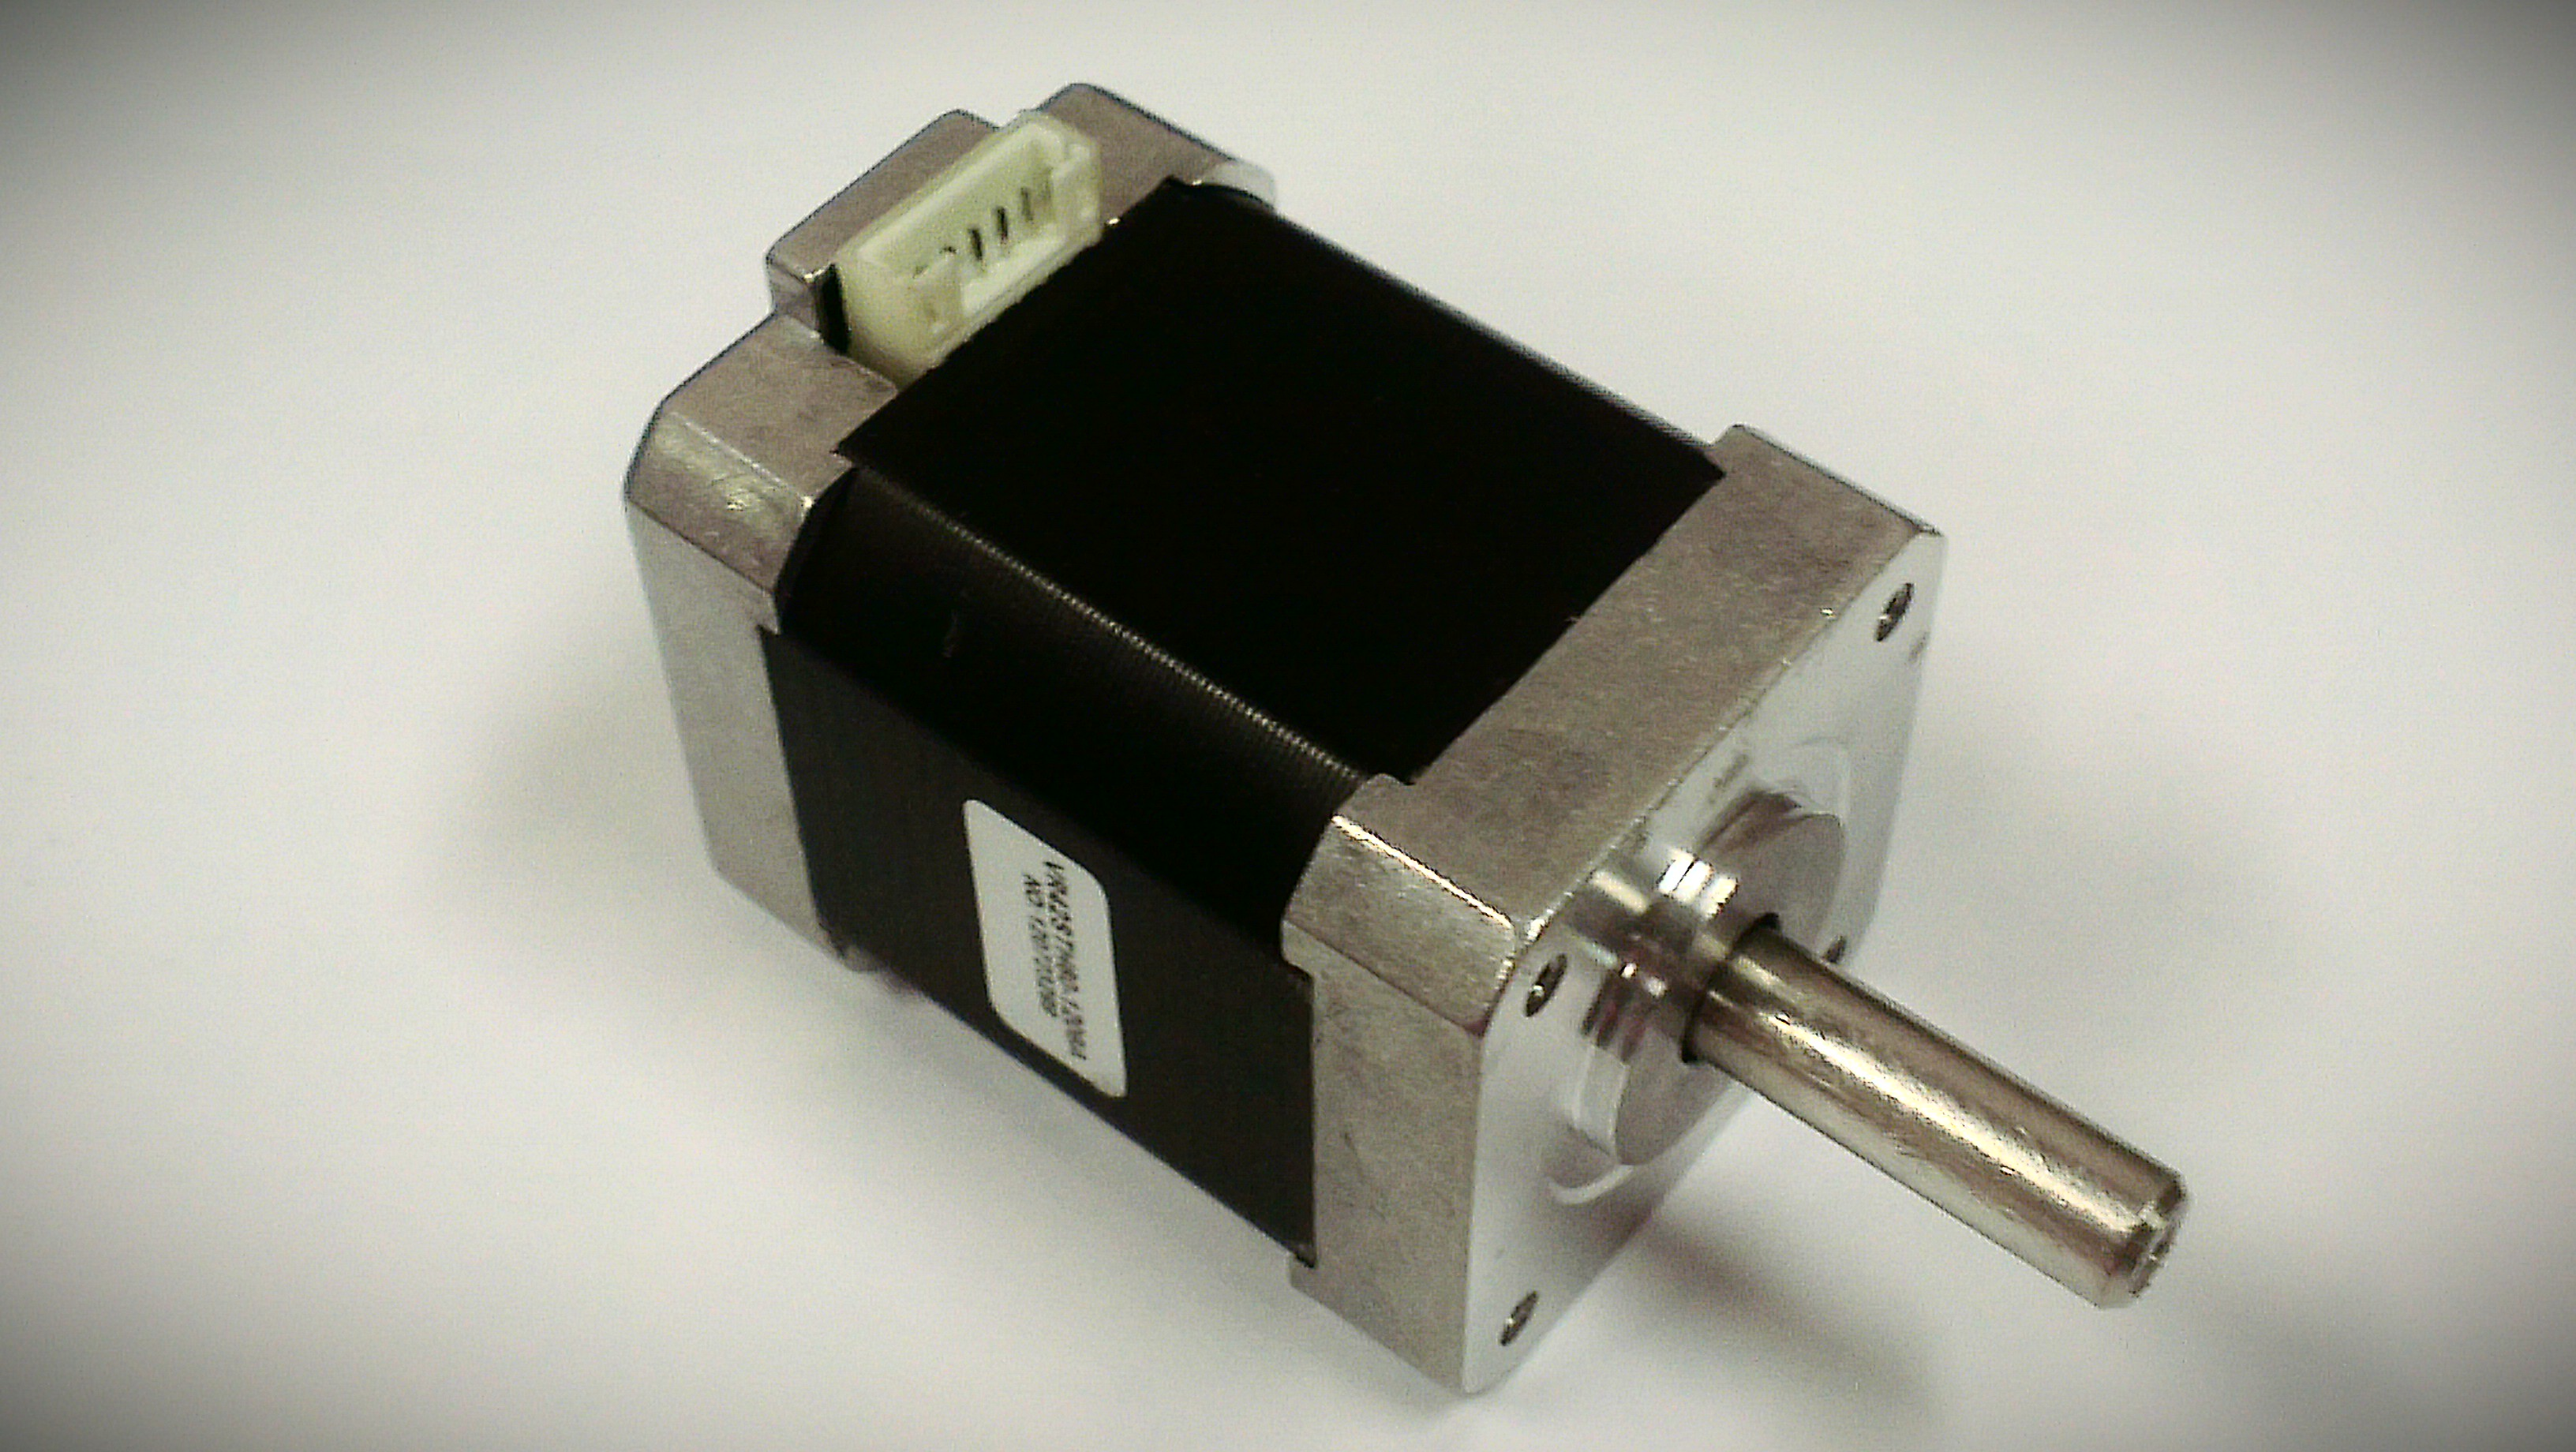
\includegraphics[width=\linewidth]{IMAG0758_1}
		\end{minipage}
	\pause
	%So the first question that arises is, What is a stepper motor? A stepper motor is a special kind of motor,
	\hfill
		\begin{minipage}[c]{0.3\textwidth}
			\begin{enumerate}
				\item <+-|alert@+> Rotates in discrete steps
				%whose rotation is divided into dicrete steps which allow precise control over its angle.
				\item <+-|alert@+> Can hold or move to a position
				%It can be commanded to hold a step or move to the next step.
			\end{enumerate}
		\end{minipage}   
\end{frame}

\subsection{Types of Stepper Motors}
\begin{frame}
	\frametitle{Types of Stepper Motors}
	\pause
	%Types
	%Steppers are mainly classified on the basis of their internal wiring. These classes are as follows.
	\begin{minipage}[c]{0.45\textwidth}
	\begin{itemize}
		\item Bipolar
			\begin{itemize}
				\item Has 4 wires
				
			\end{itemize}
	\end{itemize}
	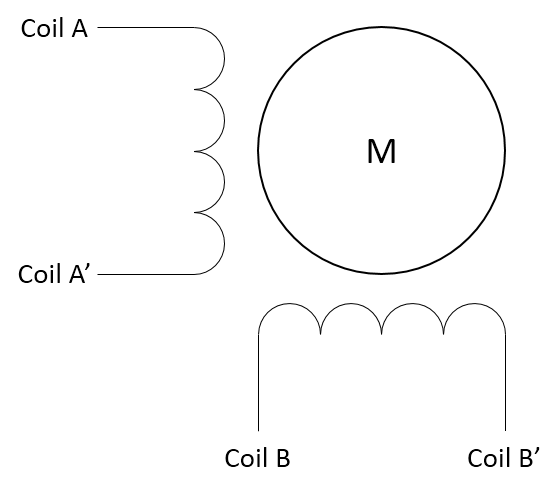
\includegraphics[width=\linewidth]{Bipolar}
	\end{minipage}
	\pause
	%Bipolar Steppers usually have 4 wires to control them and their drivers are complex		
	\begin{minipage}[c]{0.45\textwidth}
		\begin{itemize}
			\item Unipolar
				\begin{itemize}
					\item Has 5 or 6 wires
					
				\end{itemize}
		\end{itemize}
		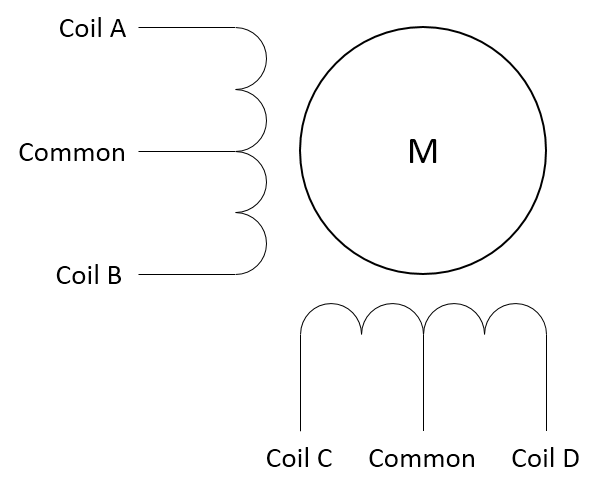
\includegraphics[width=\linewidth]{Unipolar}
	\end{minipage}
	\pause
	%Unipolar Steppers on the other hand have 5 or 6 wires and are relatively easier to drive
	
	We will use a unipolar stepper motor.
	%Since, Unipolar motors are commonly used, we will be using them in this tutorial
\end{frame}
\section{Controlling a Stepper Motor}

\subsection{Stepping sequences}

\begin{frame}
	\frametitle{Stepping sequences}
	\pause
	%Moving on to how to control a stepper motor, a stepper motor can be controlled by sending specific sequences of signals to its wires. The different stepping sequences are
	\begin{enumerate}
		\item <+-|alert@+> Wave Stepping
		%Wave Stepping
		\item <+-|alert@+> Full Stepping
		%Full Stepping
		\item <+-|alert@+> Half Stepping
		%and Half Stepping
	\end{enumerate}
	%We will now see and understand how to use each one of them.
\end{frame}

\subsection{Wave Stepping}

\begin{frame}
	\frametitle{Wave Stepping}
	\pause
	%Wave stepping
	%It involves exciting each coil turn by turn in a circular fashion.
	\begin{table}
		\begin{tabular}{c c c c c}
			\toprule
			\textbf{Step} & \textbf{Coil A} & \textbf{Coil B} & \textbf{Coil C} & \textbf{Coil D}\\
			\midrule
			1 & 1 & 0 & 0 & 0 \\
			2 & 0 & 1 & 0 & 0 \\
			3 & 0 & 0 & 1 & 0 \\
			4 & 0 & 0 & 0 & 1 \\
			\bottomrule
		\end{tabular}
		\caption{Wave stepping sequence}
	\end{table}
	%The table shows which coils are to be excited for generating the wave stepping sequence. Here a 1 denotes ON whereas a 0 denotes OFF. To rotate the stepper motor in one direction, we send the sequence, 1-2-3-4-1 and so on while for the opposite direction, we send the sequence in reverse, i.e., 4-3-2-1-4 and so on.
\end{frame}

\begin{frame}
	\frametitle{Wave Stepping (contd.)}
	%Shown here is an illustration that depicts the direction of the rotor inside a stepper motor in the wave stepping sequence. The rotor points to the excited coil at that instant. When coil A is excited, the rotor aligns itself to point to it. Next, when coil B is excited, the rotor turns to align itself again. This process repeats for the other coils.
	\begin{minipage}[c]{0.24\textwidth}
		\begin{figure}
			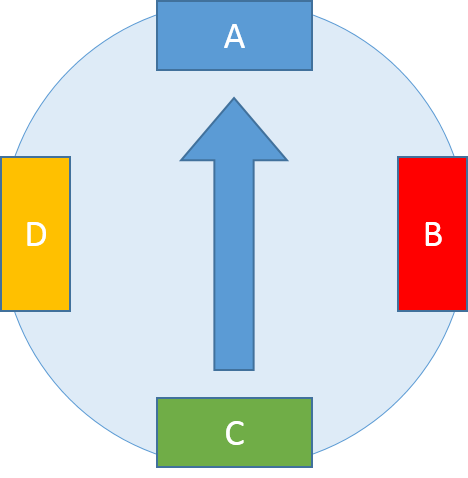
\includegraphics[width=0.9\linewidth]{step1}
		\end{figure}
	\end{minipage}
	\begin{minipage}[c]{0.24\textwidth}
		\begin{figure}
			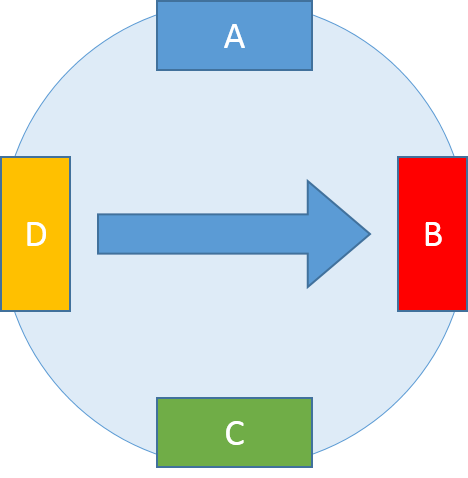
\includegraphics[width=0.9\linewidth]{step3}
		\end{figure}
	\end{minipage}
	\begin{minipage}[c]{0.24\textwidth}
		\begin{figure}
			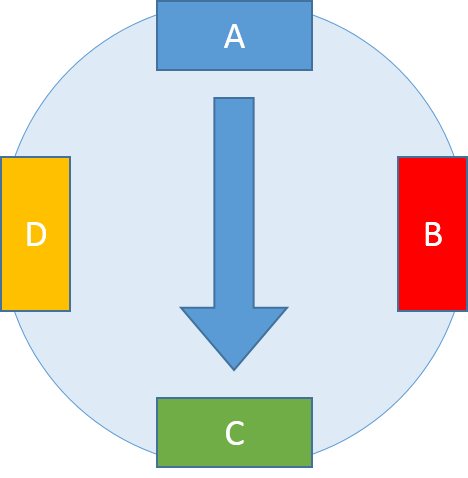
\includegraphics[width=0.9\linewidth]{step5}
		\end{figure}
	\end{minipage}
	\begin{minipage}[c]{0.24\textwidth}
		\begin{figure}
			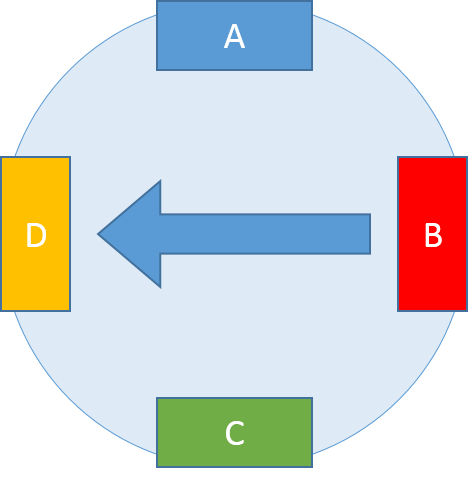
\includegraphics[width=0.9\linewidth]{step7}
		\end{figure}
	\end{minipage}
	\begin{center}
		Stepper Motor's positions in the wave stepping sequence
	\end{center}
\end{frame}

\subsection{Full Stepping}

\begin{frame}
	\frametitle{Full Stepping}
	\pause
	%Full stepping
	%It involves exciting two adjacent coils turn by turn in a circular fashion.
	\begin{table}
		\begin{tabular}{c c c c c}
			\toprule
			\textbf{Step} & \textbf{Coil A} & \textbf{Coil B} & \textbf{Coil C} & \textbf{Coil D}\\
			\midrule
			1 & 1 & 1 & 0 & 0 \\
			2 & 0 & 1 & 1 & 0 \\
			3 & 0 & 0 & 1 & 1 \\
			4 & 1 & 0 & 0 & 1 \\
			\bottomrule
		\end{tabular}
		\caption{Full stepping sequence}
	\end{table}
	%The table shows which coils are to be excited for generating the full stepping sequence. Notice that at each step exactly two coils are excited.
	%Now let's see what happens inside the motor when two coils are excited at once.
\end{frame}

\begin{frame}
	\frametitle{Full Stepping (contd.)}
	%As you can see, when two coils, say A and B are excited, the rotor settles between them. This results in a higher torque than that found in wave stepping.
	\begin{minipage}[c]{0.24\textwidth}
		\begin{figure}
			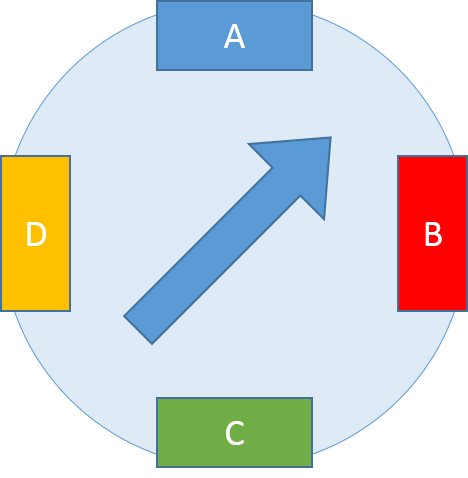
\includegraphics[width=0.9\linewidth]{step2}
		\end{figure}
	\end{minipage}
	\begin{minipage}[c]{0.24\textwidth}
		\begin{figure}
			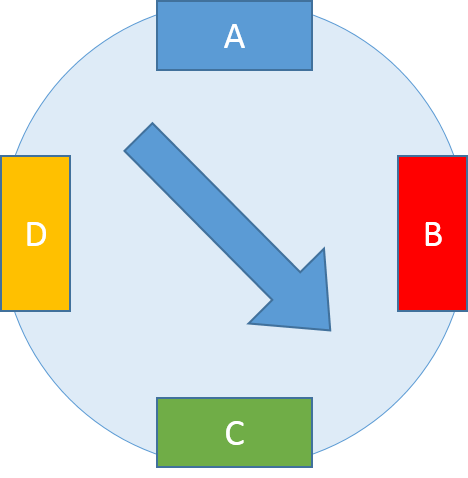
\includegraphics[width=0.9\linewidth]{step4}
		\end{figure}
	\end{minipage}
	\begin{minipage}[c]{0.24\textwidth}
		\begin{figure}
			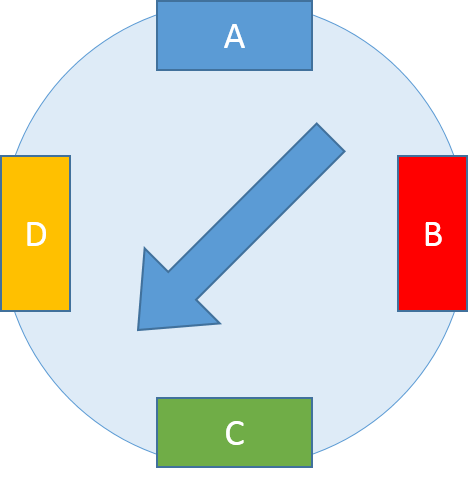
\includegraphics[width=0.9\linewidth]{step6}
		\end{figure}
	\end{minipage}
	\begin{minipage}[c]{0.24\textwidth}
		\begin{figure}
			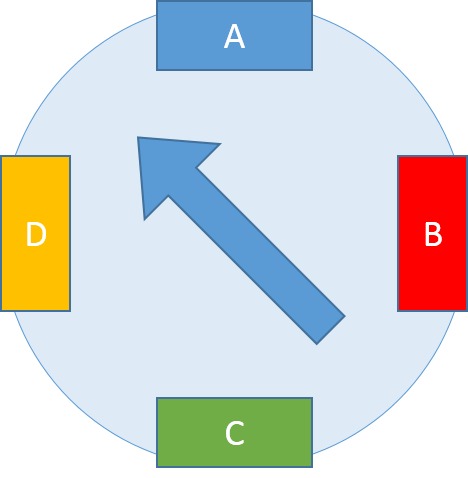
\includegraphics[width=0.9\linewidth]{step8}
		\end{figure}
	\end{minipage}
	\begin{center}
		Stepper Motor's positions in the full stepping sequence
	\end{center}
\end{frame}

\subsection{Half Stepping}

\begin{frame}
	\frametitle{Half Stepping}
	\pause
	%Half stepping
	%This stepping mode is a combination of wave and full stepping.
	\begin{table}
		\begin{tabular}{c c c c c}
			\toprule
			\textbf{Step} & \textbf{Coil A} & \textbf{Coil B} & \textbf{Coil C} & \textbf{Coil D}\\
			\midrule
			1 & 1 & 0 & 0 & 0 \\
			2 & 1 & 1 & 0 & 0 \\
			3 & 0 & 1 & 0 & 0 \\
			4 & 0 & 1 & 1 & 0 \\
			5 & 0 & 0 & 1 & 0 \\
			6 & 0 & 0 & 1 & 1 \\
			7 & 0 & 0 & 0 & 1 \\
			8 & 1 & 0 & 0 & 1 \\
			\bottomrule
		\end{tabular}
		\caption{Half stepping sequence}
	\end{table}
	%If you look closely, half stepping uses full stepping between the step positions of wave stepping. Let's see what happens inside the motor during this sequence.
\end{frame}

\begin{frame}
	\frametitle{Half Stepping (contd.)}
	%As you can see, there are 8 positions corresponding to the 8 steps shown in the previous table. It is called half stepping because it effectively halves the step angle and offers more resolution.
	\begin{minipage}[c]{0.24\textwidth}
		\begin{figure}
			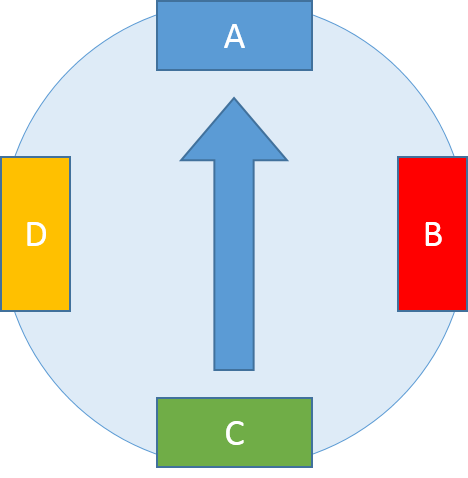
\includegraphics[width=0.9\linewidth]{step1}
		\end{figure}
	\end{minipage}
	\begin{minipage}[c]{0.24\textwidth}
		\begin{figure}
			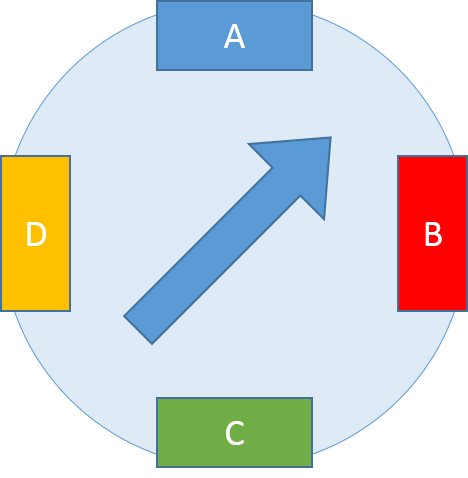
\includegraphics[width=0.9\linewidth]{step2}
		\end{figure}
	\end{minipage}
	\begin{minipage}[c]{0.24\textwidth}
		\begin{figure}
			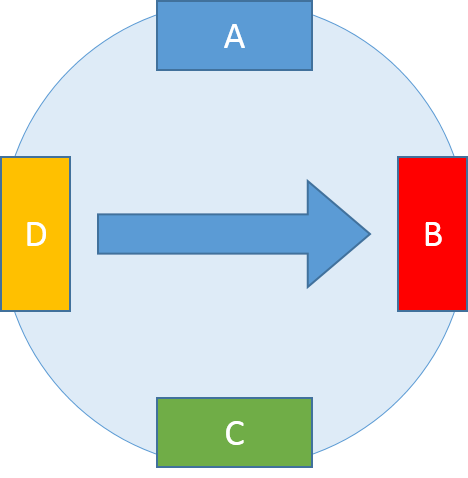
\includegraphics[width=0.9\linewidth]{step3}
		\end{figure}
	\end{minipage}
	\begin{minipage}[c]{0.24\textwidth}
		\begin{figure}
			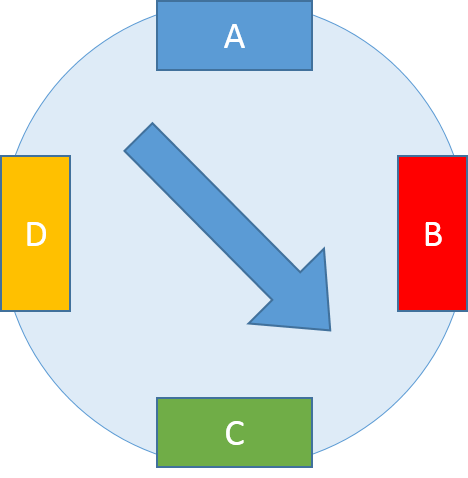
\includegraphics[width=0.9\linewidth]{step4}
		\end{figure}
	\end{minipage}
	\begin{minipage}[c]{0.24\textwidth}
		\begin{figure}
			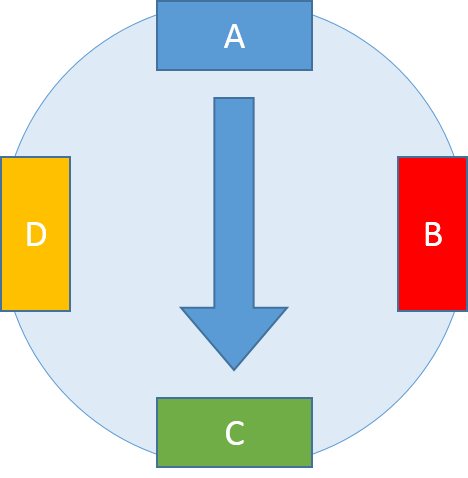
\includegraphics[width=0.9\linewidth]{step5}
		\end{figure}
	\end{minipage}
	\begin{minipage}[c]{0.24\textwidth}
		\begin{figure}
			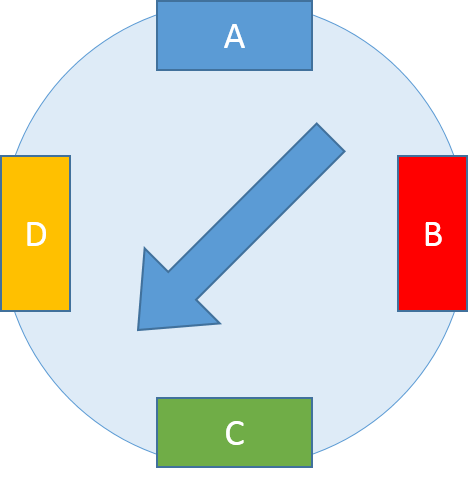
\includegraphics[width=0.9\linewidth]{step6}
		\end{figure}
	\end{minipage}
	\begin{minipage}[c]{0.24\textwidth}
		\begin{figure}
			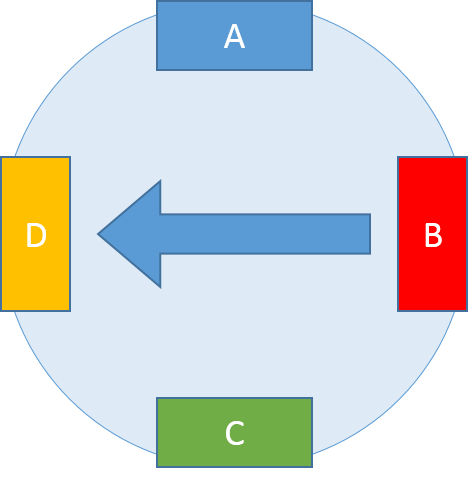
\includegraphics[width=0.9\linewidth]{step7}
		\end{figure}
	\end{minipage}
	\begin{minipage}[c]{0.24\textwidth}
		\begin{figure}
			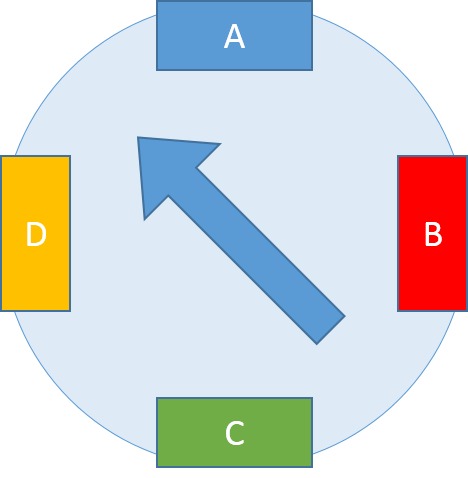
\includegraphics[width=0.9\linewidth]{step8}
		\end{figure}
	\end{minipage}
	
	\begin{center}
		Stepper Motor's positions in the half stepping sequence
	\end{center}

\end{frame}

\subsection{Comparison of stepping modes}

\begin{frame}
	\frametitle{Comparison of stepping modes}
	\pause
	%We will now see the differences and similarities between the 3 different stepping modes
	\begin{columns}[t]
		\column{.24\textwidth}
		\textbf{Stepping Mode}
		\begin{enumerate}
			\item Torque
			\item Vibration
			\item Speed
			\item Resolution
		\end{enumerate}
		
		
		\column{.24\textwidth}
		\textbf{Wave Stepping}
		\begin{enumerate}
			\item Lowest
			\item Intermediate
			\item Full
			\item Normal
		\end{enumerate}
		
		\column{.24\textwidth}
		\textbf{Full Stepping}
		\begin{enumerate}
			\item Highest
			\item Highest
			\item Full
			\item Normal
		\end{enumerate}
		
		\column{.24\textwidth}
		\textbf{Half Stepping}
		\begin{enumerate}
			\item Intermediate
			\item Lowest
			\item Halved
			\item Doubled
		\end{enumerate}
		
	\end{columns}
	%Talking about torque, since only one coil at a time is energised in wave stepping, its torque is the lowest. In full stepping, 2 coils are excited at once creating a larger attractive force resulting in a larger torque. Since half stepping excites 1 or 2 coils per step, the torque output is intermediate.
	
	%Vibration in a stepper motor increases with torque and decreases when the step angle decreases. Since wave stepping has low torque, but a step angle larger than half stepping, it has an intermediate level of vibration. Full stepping has higher torque resulting in more vibration and half stepping, due to a smaller step angle exhibits the least vibration.
	
	%Next is speed. Speed is equal to the step angle times the step frequency, since the step angle is the same for wave and full stepping, they have the same speed. For half stepping, the stepping angle is halved and thus the speed is also halved.
	
	%Resolution is fineness of control over rotational angle and is equal to the step angle. The step angle is equal for wave and full stepping while it is halved for half stepping.

\end{frame}

\section{Identifying the wires of a stepper motor}

\begin{frame}
	\begin{center}
		\textbf{\LARGE Identifying the wires of a stepper motor}
		%We will now learn how to identify the wires of a stepper motor.
	\end{center}
\end{frame}
%--------Video of practical identification of wires-----

\section{Stepper Motor Driver}

\begin{frame}
	\frametitle{Stepper Motor Driver Circuit}
	\begin{center}
		%This is the circuit diagram for the stepper motor driver
		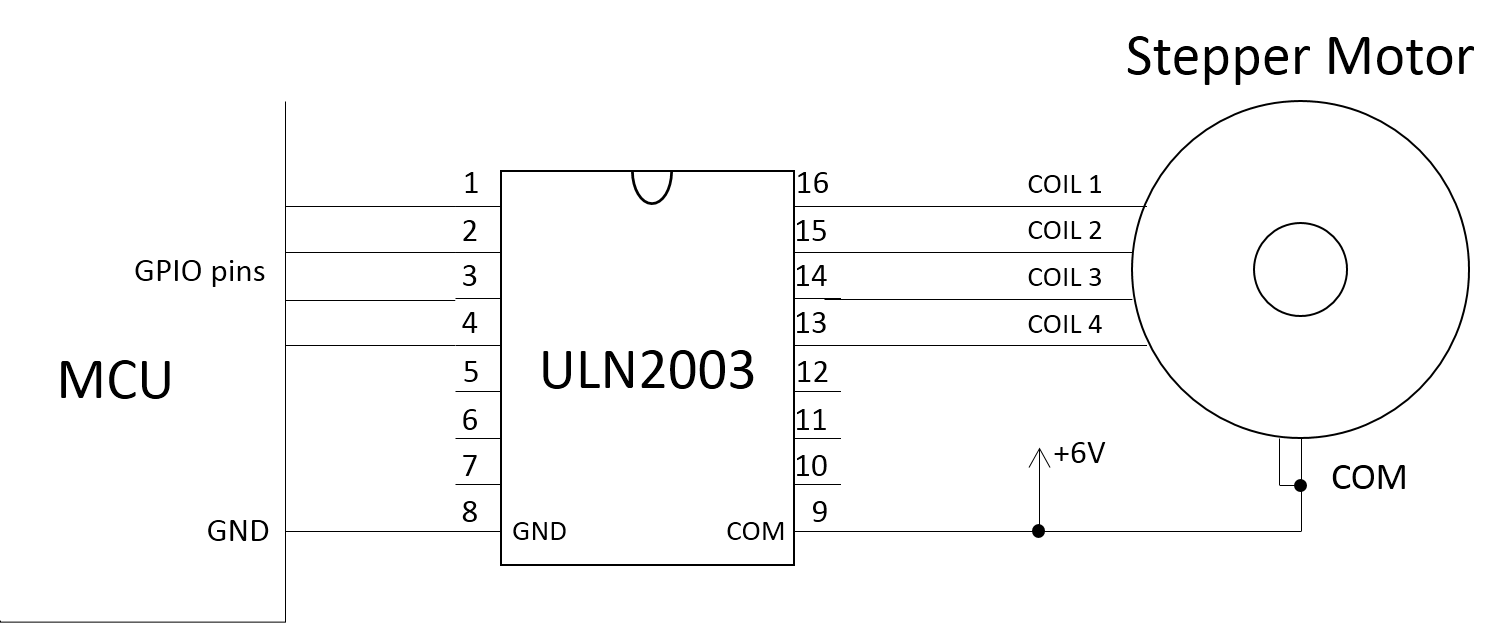
\includegraphics[width=\linewidth]{Driver}
		%The ULN2003 is a transistor array package of 7 transistors that are capable of switching 500 milli Amperes of current per transistor. The pins 1-7 are the inputs to the transistors, while the pins 16-10 are the corresponding open-collector outputs. All transistors have a commmon emitter that is connected to the ground at pin 8. The COM pin at pin 9 is connected externally to the supply voltage. The circuit is basically used to drive the stepper's high current windings by a microcontroller's General Purpose IO pins.
	\end{center}
\end{frame}

\section{Interfacing with ATmega2560}

\subsection{GPIO pins}
\begin{frame}
	\frametitle{Interfacing with ATmega2560}
	\framesubtitle{GPIO pins}
	%We will now discuss how to interface the Firebird V robot with the stepper motor using this circuit
	\pause
	\begin{center}
		\begin{table}
			\begin{tabular}{c c c}
			\toprule
			\textbf{Expansion Slot pin} & \textbf{MCU pin} & \textbf{Connected to}\\
			\midrule
			17 & PL7 & ULN2003 pin 1 \\
			18 & PL6 & ULN2003 pin 2 \\
			19 & PD1 & ULN2003 pin 3 \\
			20 & PD0 & ULN2003 pin 4 \\
			23 & GND & ULN2003 pin 8 \\
			\bottomrule
			\end{tabular}
			\caption{GPIO pins used}
		\end{table}
		
		%These are the Firebird V robot's expansion slot pins which we are going to use to connect to the driver circuit shown previously.
		%Expansion slot pin 17 i.e., PL7 is connected to the ULN2003 driver IC's pin 1
		%Expansion slot pin 18 i.e., PL6 is connected to the ULN2003 driver IC's pin 2
		%Expansion slot pin 19 i.e., PD1 is connected to the ULN2003 driver IC's pin 3
		%Expansion slot pin 20 i.e., PD0 is connected to the ULN2003 driver IC's pin 4
		%Expansion slot pin 23 i.e., Ground is connected to the ULN2003 driver IC's Ground on pin 8
		\pause
		\begin{figure}
			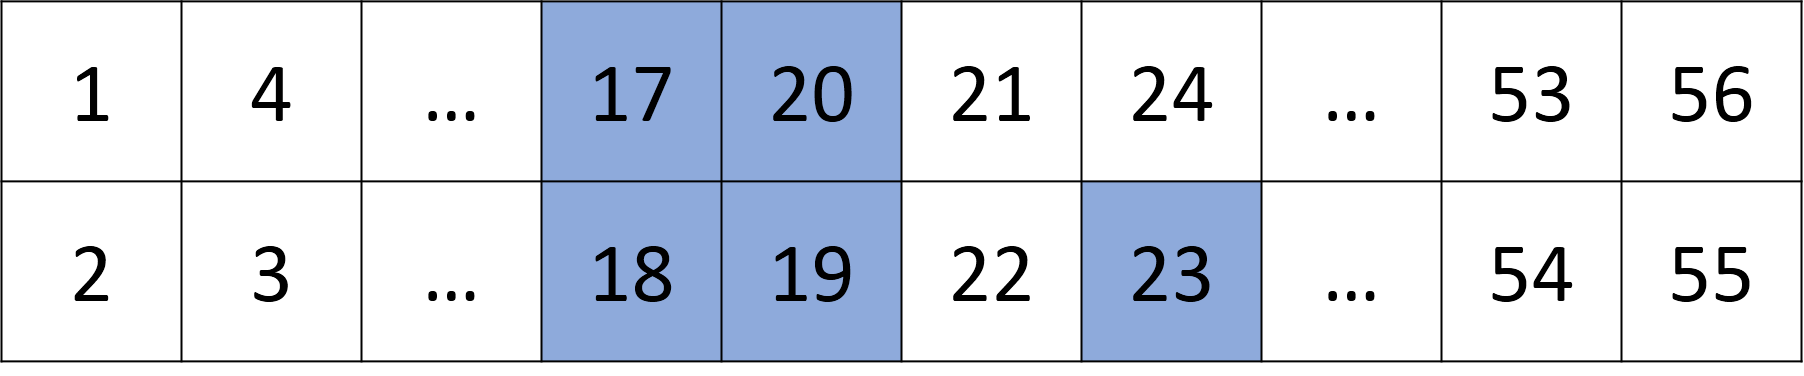
\includegraphics[width=0.5\linewidth]{pinnumbering}
			\caption{Pin numbering on the expansion slot}
		\end{figure}
		%The pins are numbered on the slot as shown in the figure. Note the unusual snake-like numbering of the expansion slot. Pins 5-16 and 25-52 are not shown for clarity. We will be using the pins 17, 18, 19, 20 and 23.
	\end{center}
\end{frame}

\subsection{Timer Configuration}

\begin{frame}
	\frametitle{Interfacing with ATmega2560}
	\framesubtitle{Timer Configuration}
	%Now for an example, we will be rotating the stepper motor in one direction at a fixed speed for a complete revolution and then change its direction and repeat the process in the opposite direction. For this, we can either use delays between steps or we can use one of the AVR timers for the delays. For a challenge, let's talk about achieving this with the second method.
	\pause
	\begin{enumerate}[$\checkmark$]
		\item <+-|alert@+> Time period of stepping = 3.333 ms $\Rightarrow$ Frequency = 300 Hz
		%Moving the stepper a single step every 3.333 ms means running the motor at a step frequency of 300Hz
		\item <+-|alert@+> 16-bit Timer1 in CTC mode $\Rightarrow$ WGM13:0 = 4 (bin: 0100)
		%To achieve this, we select the 16-bit Timer1 and run it in CTC mode i.e., Clear on Timer Compare Match by setting the Waveform Generation Mode bits to 0100.
		\item <+-|alert@+> Prescaler = 1
		%We will set the prescaler to 1 as we do not need the timer clock to be divided by any factor.
		\item <+-|alert@+> Timer frequency = 300 Hz. So, $$ OCR1A = TOP = \frac{f_{CLK}}{f_{timer}} - 1 = \frac{14745600}{300} - 1 = 49151$$
		%Since the required frequency is 300Hz, we set the TOP value to 49151 calculated by this formula. The timer's OCR1A register value is used as the TOP value in CTC mode.
		\item <+-|alert@+> Compare interrupt enabled
		%Finally we enable the compare match interrupt to step the motor in the Interrupt Service Routine every time a compare match occurs.
	\end{enumerate}
\end{frame}

\subsection{Code}
\begin{frame}[shrink = 2,fragile]
	\frametitle{Interfacing with ATmega2560}
	\framesubtitle{Code}
	%Now that we have understood how to use the timer for our purpose, let's have a look at the code.
	\pause
	\begin{block}<2->{\#include}
		\begin{semiverbatim}
			\scriptsize{
\#include <avr/io.h>
\#include <avr/interrupt.h>
\#include "stepper.h"
			}
		\end{semiverbatim}
	\end{block}
	%This is a list of headers to be included, which are: avr/io.h, avr/interrupt.h and a custom header called stepper.h that contains the functions for controlling the GPIO pins of the stepper in different step modes.
	\begin{block}<3->{Interrupt Service Routine}
		\begin{semiverbatim}
			\scriptsize{
ISR(TIMER1\_COMPA\_vect)
\{
    wave\_step(direction);
    stepcount++;
    if(stepcount > 200) \color{comment}//Change direction every revolution\color{black}
    \{
        direction *= -1;
        stepcount = 0;
    \}
\}
			}
		\end{semiverbatim}
	\end{block}
	%The interrupt service routine is called whenever a compare match occurs and we will use this to make a single step. direction here is a global variable that is initially set to +1 and is changed to -1 after every 200 steps by the following code which increments stepcount in each call of the ISR and changes direction from +1 to -1 and vice versa if the stepcount exceeds 200. It then resets the stepcount to 0.
	%The stepper motor we use, completes a revolution in 200 steps. Modify this value if your stepper motor's steps per revolution value is different.
\end{frame}

\begin{frame}[shrink = 2,fragile]
	\frametitle{Interfacing with ATmega2560}
	\framesubtitle{Code (contd.)}
	%1:
	%Moving on to the main function, first we initialize the IO ports for the stepper motor.
	%2: (pause)
	%Then, we setup Timer1 with the configuration we decided upon. To do this, we first temporarily disable all interrupts while setting up and set Timer1 to work in CTC mode by setting WGM bits to 0100 in the TCCR1B register. Only WGM12 is set as the other WGM bits are by default zero. Then the Output Compare Match Interrupt for Timer1 is enabled by setting bit OCIE1A in the TIMSK1 register. Finally we re-enable all the interrupts after initialisation
	%3: (pause)
	%We then set the TOP value in the OCR1A register using the given formula. Here F_CPU and SPEED are previously defined constant whose values are 14745600 and 300 respectively.
	%4: (pause)
	%Then we finally start the timer by setting the prescaler to 1 through the CS12, CS11 and CS10 bits in the TCCR1B register.
	%5: (pause)
	%Then we handover the job to the interrupts and thus let the processor go into an infinite loop.
	\begin{block}<1->{Main Program}
		\begin{semiverbatim}
			\scriptsize{
int main(void)
\{
    stepper\_port\_init(); \color{comment}//Initialize ports\color{black}
\pause
    cli(); \color{comment}//Clear global interrupts\color{black}
    TCCR1B |= (1 << WGM12); \color{comment}//CTC mode (WGM13:0 = 0100)\color{black}
    TIMSK1 |= (1 << OCIE1A); \color{comment}//Enable CTC interrupt\color{black}
    sei(); \color{comment}//Enable global interrupts\color{black}
\pause
    OCR1A = (F\_CPU / SPEED) - 1; \color{comment}//Set TOP\color{black}
\pause
    \color{comment}//Prescalar = 1\color{black}
    TCCR1B |= ((0 << CS12) | (0 << CS11) | (1 << CS10));
\pause
    while(1);
\}
			}
		\end{semiverbatim}
	\end{block}
\end{frame}

%----------Show code in Atmel Studio------------
%----------Show working video of the code-------
%So by now we have successfully understood the control of stepper motors and how to interface a stepper motor with the ATmega2560 based Firebird V robotics platform. You may modify the code to experiment with different stepping modes and speeds or by setting it to specific angles, etc.

\begin{frame}
	\begin{center}
		\textbf{\LARGE Thank You!} \\
		\vspace{20pt}
		\scriptsize Send your queries to: 
		\href{mailto:helpdesk@e-yantra.org} {\color{blue}helpdesk@e-yantra.org \color{black}}
	\end{center}
	%With this we have reached the end of this video tutorial. Thank you for listening! For any doubts or suggestions feel free to mail them at helpdesk@e(hyphen)yantra(dot)org
	%This is Joel Pinto signing off!
\end{frame}

\end{document}